\section{Solving SPJM Problem}
\label{sec:solve-spjm-problem}
There are already a considerable number of research findings and solutions for the SPJ problem \cite{}.
Given that the main difference between SPJM and SPJ lies in the matching operator, in addressing the SPJM problem, solutions from the SPJ problem can be referenced.
In this section, we focus on the method to deal with the matching operators.
Firstly, an intuitive method is presented and then an advanced method based on matching decomposition is proposed.
For simplicity, the pattern graph given in matching operators are assumed to be connected in this section.

\subsection{Intuitive Method}
\label{sec:intuitive-method}
A straightforward method for processing the matching operator is to transform it into an SPJ query, and then optimize the query with relational optimizers.
Specifically, given a matching operator $\mathcal{M}(GR, \mathcal{P})$, according to the \rgmapping, vertices and edges in $\mathcal{P}$ have corresponding relations.
Then, the matching operator can be converted to a sequence of join operators between these relations.
Please note a matching operator is always followed by a projection operator $\widehat{\pi}_{attr}$ to extracts specified attributes from the output graph relation.
After the matching operator is converted to an SPJ query, the projection operation should be modified accordingly to project the output relation onto the corresponding attributes.
The following lemma indicates that matching operators can always be transformed to SPJ queries losslessly.
Therefore, this method is applicable across different scenarios.

\todo{matching operator with $\widehat{\pi}$}
\begin{lemma}
    \label{lemma:spjm-to-spj}
    The matching operator can be losslessly converted to an SPJ query.
\end{lemma}
\begin{proof}
    We first focus on the matching operators under the semantics of homomorphism and prove the theorem by induction.
    % We begin with matching operators with homomorphic semantics, and prove the theorem using induction.
    Given a matching operator $\matching(GR, \pattern)$, vertices and edges are called elements in $\pattern$.
    Then, induction is conducted on the number of elements in $\mathcal{P}$.
    
    When there is only one element in $\mathcal{P}$, e.g., $\mathcal{P}=(u:\text{Person} \{\cdots\})$, such a matching operator can be expressed with a relation and a selection operator, e.g., $\sigma_d(Person)$.
    The SPJ query has the same meaning as the matching operator, since all the attributes of vertices labeled $Person$ are contained in the output relation.
    Please note that if there are more constraints on the element (e.g., the returned person should be at least 18 years old), more constraints can be specified with the selection operators.

    Suppose a matching operator $\matching(GR, \pattern_x)$, whose pattern graph contains $x$ elements ($x \leq n$), can be expressed with SPJ operators.
    Denote the sequence of SPJ operators by $\mathcal{E}_{\mathcal{P}_x}$.
    When there are $n+1$ elements in the pattern graph of a matching operator $\matching(GR, \mathcal{P}_{n+1})$, let $v$ be a vertex in $\mathcal{P}_{n+1}$, and $e_1, \cdots, e_k$ are the edges adjacent to $v$. %connecting $v$ with the other vertices in $\mathcal{P}$.
    $\mathcal{P}_s$ is the pattern obtained by removing $v$ and $e_1, \cdots, e_k$ from $\mathcal{P}_{n+1}$.
    $\mathcal{P}_s$ contains $s$ elements and $\matching(GR, \mathcal{P}_s)$ can be expressed with $\mathcal{E}_{\mathcal{P}_s}$.
    Then, $\matching(GR, \mathcal{P}_{n+1})$ can be expressed with SPJ operators as follows:
    \begin{equation*}
        \mathcal{E}_{\mathcal{P}_s} \Join R_{el_1} \Join \cdots \Join R_{el_k} \Join R_{vl},
    \end{equation*}
    where $vl$ is the label of $v$, $el_1, \cdots, el_k$ are labels of $e_1, \cdots, e_k$, $R_{l}$ is the relation corresponding to vertices or edges labeled $l$ according to the \rgmapping.
    In conclusion, adopting the homomorphism semantics, the matching operator can be expressed with SPJ operators.

    Furthermore, when the matching operator adopt other semantics (e.g., isomorphism), it is straightforward to add some constraints on the elements with selection operators.
    For instance, when the isomorphism semantics is adopted, constraints should be added to ensure that different vertices in the pattern graph match with different vertices in the database.
    Therefore, the theorem is correct. 
\end{proof}

Some existing works have adopted this idea and implemented translators to convert SPJM queries to SPJ queries.
Two typical products include Apache Age \cite{apache-age} and DuckPGQ \cite{DuckPGQ,DuckPGQ-VLDB}.

\begin{example}
    For the SPJM query shown in Fig.~\ref{fig:spjm}, it can be transformed to the SPJ query as follows:
    \begin{equation*}
        \pi_A(\sigma_d(\pi_{A'}(Person \Join Likes \Join Message \Join Likes \Join Person) \Join Place))
    \end{equation*}
    Then, this SPJ query can be optimized with relational optimizers.
\end{example}

\subsection{Decomposition-based Method}
The straightforward method proposed in Sec.~\ref{sec:intuitive-method} is inefficient, because tables representing vertices and edges are treated equally by relational optimizers and worst-case optimality cannot be guaranteed.
Besides, in the sequence of join operators, a table representing edges may not be joined with tables representing its adjacent vertices.
Then, some graph-level optimizations cannot be applied.

Therefore, in this subsection, we present a decomposition-based method to process matching operators.
In detail, given a matching operator $\matching(GR, \mathcal{P}_0)$ in an SPJM query, it is decomposed into two new matching operators $\matching(GR, \mathcal{P}_1)$ and $\matching(GR, \mathcal{P}_2)$ connected with a join operator $\widehat{\Join}$, following \cite{huge}.
Specifically, $\mathcal{P}_1$ and $\mathcal{P}_2$ should satisfy: 
(1) $V_{\mathcal{P}_0} = V_{\mathcal{P}_1} \cup V_{\mathcal{P}_2}$,
(2) $E_{\mathcal{P}_0} = E_{\mathcal{P}_1} \cup E_{\mathcal{P}_2}$,
(3) $V_{\mathcal{P}_1} \cap V_{\mathcal{P}_2} \neq \emptyset$,
(4) $E_{\mathcal{P}_1} \cap E_{\mathcal{P}_2} = \emptyset$.
Please note that $\widehat{\Join}$ and $\Join$ is almost identical, except for the fact that $\widehat{\Join}$ joins two graph relations and outputs a new graph relation.

The new matching operators can be further decomposed.
To prevent the matching operator from being decomposed indefinitely, it is necessary to define a type of matching operator that cannot be decomposed.
In this paper, such a matching operator is called a minimum matching component (abbr.~MMC).

\begin{definition}[Minimum Matching Component, abbr.~MMC]
    A matching operator is called a minimum matching component iff the matching of the pattern has a specific physical implementation according to the optimizer and the matching operator will not be further decomposed.
\end{definition} 

Therefore, decomposing the matching operators recursively can finally result in a tree, whose leaf nodes are MMCs.
To ensure worst-case optimality, in the process of decomposition, the pattern graph of each decomposed matching operator should be an induced subgraph of $\mathcal{P}_0$.
The generated tree is called a decomposition tree and it is actually a logical plan of the matching operator.
\modify{Without loss of generality, the left-deep join order is employed on the tree.}

Then, it is crucial to identify which matching operators to treat as MMCs.
We adopt the definition of \emph{complete star} from \cite{huge} and utilize 
Specifically, suppose $\matching(GR, \mathcal{P})$ is decomposed into $\matching(GR, \mathcal{P}_1)$ $\widehat{\Join}$ $\matching(GR, \mathcal{P}_2)$, $\mathcal{P}_2$ is called a complete star iff $\mathcal{P}_2$ is a star $(v_r; \mathcal{L})$ and $\mathcal{L} \subseteq E_{\mathcal{P}_1}$, where $v_r$ is the root and $\mathcal{L}$ is the set of its leaf vertices.
Inspired by HUGE \cite{huge} and GLogS \cite{GLogS}, matching operators located on the right subtree of the join operator with complete stars as the pattern graphs are the MMCs in this paper.

Besides, a matching operator located on the left subtree of the join oeprator is an MMC iff its pattern graph is an edge (i.e., one edge and its adjacent two vertices).

\begin{figure}
    \centering
    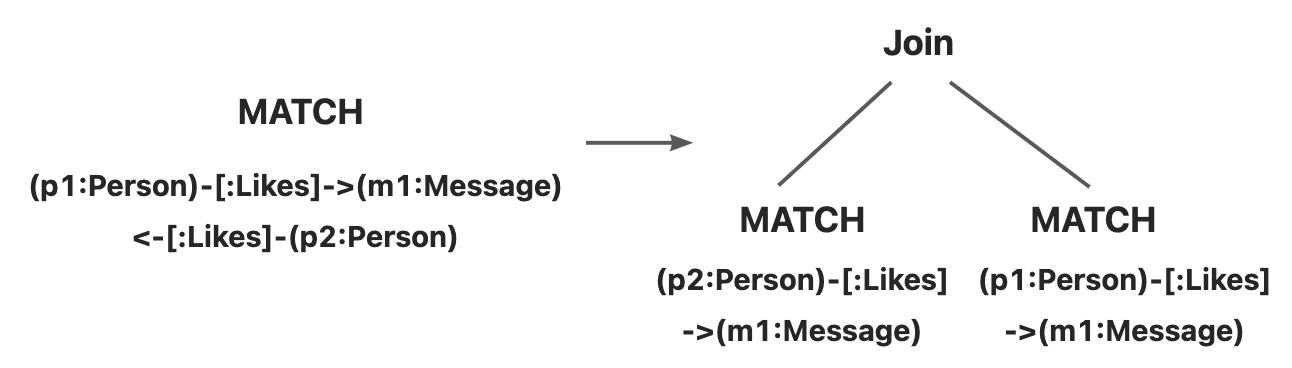
\includegraphics[width=.8\linewidth]{./figures/match-decompose.png}
    \caption{Decomposion of the match operator in the SPJM query shown in Fig.~\ref{fig:spjm}.}
    \label{fig:match-decomposition}
\end{figure}

\begin{example}
    Given the matching operator in Fig.~\ref{fig:spjm}, it is decomposed into two matching operators as shown in Fig.~\ref{fig:match-decomposition}.
    For the right matching operator, because its pattern is a complete star $(p_1, \{m_1\})$, the operator is an MMC.
    For the left matching operator, as its pattern is an edge pattern, it is also an MMC.
    Therefore, the decomposition tree cannot be further decomposed and is a logical plan.
\end{example}

\subsection{Comparision of Search Space}
\label{sec:compare-search-space}

The search space complexity of the decomposition-based method differs greatly from that of the straightforward method for optimization.
In this subsection, we compare the complexities with theoretically analysis.
For simplicity, we focus on the search space of join order optimization and the selection and projection operators are omitted.

Specifically, for the straightforward method, the matching operator is transformed into a sequence of join operators between relations representing vertices and edges.
Therefore, the join order can be optimized with any relational optimizer.
Since Calcite \cite{calcite,columbia} is one of the most widely adopted optimizers for relational databases, it is utilized as a representative of relational optimizers in this analysis.

For the decomposition-based method, given a matching operator $\matching(GR, \pattern)$ in an SPJM query, the outputs of the join operators in the decomposition tree are all induced subgraphs of $\pattern$.
This is consistent with the requirements of GLogS \cite{GLogS}, which is one of the state-of-the-art graph optimizers.
Therefore, the obtained plan is optimized with GLogS.

The complexity of optimization with Calcite is analyzed first.
\begin{theorem}
    \label{theorem:complexity-of-calcite}
    Given $n + m$ relations joined together, $n$ of them representing vertcies and $m$ representing edges, the complexity of join order optimization with Calcite is at least $O(4^{m+n-1})$.
\end{theorem}
\begin{proof}
    We first construct a graph with these $n + m$ relations.
    Specifically, each relation corresponds to a vertex in this graph, and if there is a join condition w.r.t.~two relations, there is an edge between the corresponding vertices.
    To avoid cross product, everytime two relations are joined together, there should be join conditions between them.
    Therefore, the join order can be represented as a spanning tree in the graph.
    By computing the number of physical plans can be generated according to each spanning tree, the total number of physical plans can be obtained.
    
    In this proof, we compute the number of physical plans for one spanning tree, and this number is a lower bound of the number of physical plans that can be generated.

    We start with a spanning tree with $k$ edges ($k \geq 1$), which has only one leaf node (i.e., it is a path).
    Then, the number of logical plans corresponding to the spanning tree is
    \begin{equation*}
        \begin{split}
            c_l(k) & = 2 * (c(0)c(k-1) + c(1)c(k-2) + \cdots + c(k-1)c(0)) \\
            & = 2\Sigma_{i=0}^{i=k-1}c(i)c(k-1-i), \\
            & \text{where } c_l(0) = 1.
        \end{split}
    \end{equation*}
    With the generating function, it is obtained that 
    \begin{equation*}
        \begin{split}
            c_l(k) & = \frac{2^k}{k+1}C(2k, k) \geq \frac{2^k}{k+1}\frac{2k \times \cdots \times (k+1)}{k \times \cdots \times 1} \\
            & \geq \frac{2^k}{k+1}2^{k-1}(k+1) = \frac{4^k}{2}
        \end{split}
    \end{equation*}

    For any spanning tree $T$ with $k = m + n - 1$ edges, denote the longest path in the tree by $p_1$, and its length is $P_1 = |p_1|$.
    By removing the path (i.e., edges in $p_1$) from $T$, we can obtain a new subgraph $T_1$.
    Similarly, the longest path in $T_1$ that intersects with the already removed paths (i.e., $p_1$) is obtained and denoted by $p_2$, with $P_2 = |p_2|$.
    After that, $p_2$ is removed from $T_1$ and subgraph $T_2$ is obtained.
    For $p_1$ and $p_2$, since they are both paths, the numbers of logical plans corresponding to them are $c_l(P_1)$ and $c_l(P_2)$, respectively.
    Without loss of generality, suppose $p_1$ and $p_2$ intersects at vertex $v_i$, and then, $v_i$ appears in each logical plan corresponding to $p_1$.
    Then, by replacing $v_i$ with the plans corresponding to $p_2$, respectively, $c(p_1 \cup p_2) \geq c_l(P_1)c_l(P_2)$ plans are obtained, where $c(t)$ is the number of logical plans corresponding to tree $t$ and $c(t) = c_l(k)$ when $t$ is a path with $k$ edges.

    As $T$ is a tree, by repeatedly finding and removing the paths as above, all the edges in $T$ are finally removed.
    Let the number of paths removed be $s$, we have 
    \begin{equation*}
        \begin{split}
            c(T) & = c(p_1 \cup \cdots \cup p_s) \geq c_l(P_1) \cdots c_l(P_s) \\
            & \geq \frac{4^{P_1 + \cdots + P_s}}{2^s} = \frac{4^{m + n - 1}}{2^s} \geq 2^{m+n-1}.
        \end{split}
    \end{equation*}
    
    %Thus, the number of logical plans w.r.t.~a spanning tree is 
    %\begin{equation*}ƒ
    %    \frac{2^{m+n-1}}{m+n}C(2m+2n-2, m+n-1) \geq \frac{4^{m+n-1}}{m+n}.
    %\end{equation*}
    

    Thus, the number of physical plans is at least $2^{m+n-1}t^{m+n-1} \geq 4^{m+n-1}$, so is the complexity of join order optimization with Calcite.
   
    In conclusion, Theorem \ref{theorem:complexity-of-calcite} is correct.
\end{proof}

Then, we analyze the complexity of optimization with GLogS.

\begin{theorem}
    \label{theorem:complexity-of-glogue}
    Given a matching operator whose pattern graph consists of $n$ vertices and $m$ edges, the complexity of join order optimization with GLogS is smaller than $3^n$.
\end{theorem}
\begin{proof}
    Since the considered patterns are all induced subgraphs in GLogS, the complexity of join order optimization is not related to the number of edges (i.e., $m$).
    Then, the join order optimization problem is reduced to a variant of the shortest path problem, and the complexity is $O(\mathcal{E})$, where $\mathcal{E}$ is the number of edges in GLogue.
    In detail, 
    \begin{equation*}
        \begin{split}
            %O(\mathcal{E}) & = C(n, n-1)*(2^{n-1}-1) + C(n, n-2) * (2^{n-2}- 1) \\
            %& + \cdots + C(n, 1) * (2^1 - 1) \\
            O(\mathcal{E}) & = \Sigma_{i=1}^{i=n-1}C(n, i)(2^i - 1) = 3^n - 2^{n+1} +1 < 3^n.
        \end{split}
    \end{equation*}
    
    In conclusion, Theorem \ref{theorem:complexity-of-glogue} is correct.

\end{proof}

Based on the complexity analysis in Theorem \ref{theorem:complexity-of-calcite} and Theorem \ref{theorem:complexity-of-glogue}, it is found that when there is only a matching operator, 
\begin{equation*}
    \begin{split}
        \frac{\text{Complexity of Calcite}}{\text{Complexity of relgo}} & > O(\frac{4^{m+n-1}}{3^n}) = O(4^{m-1}(\frac{4}{3})^n).
    \end{split}
\end{equation*}
Therefore, it suggests that GLogS is exponentially faster than Calcite in optimizing matching operators.
It also illustrates the superiority of the decomposition-based method.

\iffalse
\section{Solutions for SPJM Problem}
Two techniques can be applied to assist in solving the SPJM problem.
Since the inputs of matching operators include a graph relation that can be represented as a property graph and a pattern, this process can be regarded as querying on graphs.
Then, the graph structure can be leveraged to generate better plans.
Moreover, in a graph, vertices and edges do not have to be joined one by one and the results of specific substructures can be obtained more efficienctly.
In this section, we first introduce the concepts of the above techniques, and then present different types of methods for solving the SPJM problem.

\subsection{Graph Structure}

The definition of graph structure is as follows.

\begin{definition}[Graph Structure, abbr.~GS]
    Graph structure refers to the connectivity relationships between vertices and edges within the graph, which can be stored in graph indices in varied data structure such as adjacent lists.
\end{definition}

With graph structure, tables can be joined more efficiently.
For example, when two tables representing persons and friendships respectively are joined together, the rows that can be joined are quickly located using graph indices.
Therefore, when graph indices are available, using join methods that can leverage graph indices is a more efficient choice.

\subsection{Graph Matching Decomposition}

A matching operator can be decomposed into two new matching operators.
By joining the results of the new matching operators, the results of the original matching operator can be obtained.
Decomposing the matching operator recursively can result in a tree, which is called the match scanning plan.
Each tree node represents an operator.
\textbf{Without loss of generality, the left-deep join order is employed on the tree}.
Each internal node represents an operator including the join, selection, and projection operator.
Please note that these operators in the tree always map graph relations to graph relations, because in the matching process, graph elements are the smallest units that operators can manipulate.

For internal nodes representing join operators, they are generated when matching operators are decomposed.
Suppose a matching operator $TN_0 = \mathcal{M}(GR, \mathcal{P}_0)$ is decomposed into two child operators, i.e., $TN_1 = \mathcal{M}(GR, \mathcal{P}_1)$ and $TN_2 = \mathcal{M}(GR, \mathcal{P}_2)$.
Denote the sets of vertices and edges in a pattern $\mathcal{P}$ by $\mathcal{P}.V$ and $\mathcal{P}.E$, respectively.
Then, we have $\mathcal{P}_0.V = \mathcal{P}_1.V \cup \mathcal{P}_2.V$, $\mathcal{P}_0.E = \mathcal{P}_1.E \cup \mathcal{P}_2.E$, $\mathcal{P}_1.V \cap \mathcal{P}_2.V \neq \emptyset$, and $\mathcal{P}_1.E \cap \mathcal{P}_2.E = \emptyset$.
After $TN_0$ is decomposed, it is transformed to an internal node representing the join operator, with $TN_1$ and $TN_2$ being its child nodes.


Each leaf node of the match scanning plan is a minimum matching component, and the definition is as follows.

\begin{definition}[Minimum Matching Component, abbr.~MMC]
    A matching operator is called a minimum matching component iff the matching of the pattern has a specific physical implementation according to the optimizer and the matching operator will not be further decomposed.
\end{definition}

In the process of decomposing the matching operator, an important point is the order in which the nodes and edges are decomposed each time.
In other words, it is crucial to determine the order of the joins to generate the pattern specified in the original matching operator.
Therefore, optimizers are applied to optimize the match scanning plan.
In this paper, optimizers utilized in relational databases (e.g., Calcite) are called relational optimizers and those applied in graph databases (e.g., GLogS) are called graph optimizers.

For relational optimizers, the MMCs are matching operators whose patterns only contain a vertex or an edge.
Then, the physical implementation of such matching operators is scanning the tables of the corresponding vertices or edges, respectively.
Therefore, for relational optimizers, the matching operator will be replaced with selection operators, projection operators, and a sequence of join operators between tables representing vertices and edges.

For graph optimizers, the MMCs are more diverse.
Following the idea of StarJoin \cite{starjoin,huge}, matching operators whose patterns consist of a vertex, an edge, or a complete star are considered as MMCs.
Here, the pattern consisting of an edge actually contains the edge and its adjacent two vertices.
A complete star is a special structure on a graph.
Let $TL = \mathcal{M}(GR, \mathcal{P})$ be an MMC, which is also a leaf node of the tree, and $\mathcal{P}$ is a complete star.
Also, denote the parent node of $TL$ by $Join_{TL}$.
A complete star is a tree of depth one with at least three vertices, whose root is called the core, while the other nodes are called the outsiders.
For each outsider $v_o$ of a complete star, $v_o$ should exist in the pattern of matching operators in $Join_{TL}$'s left subtree.
Besides, $TL$ should be the right subtree of $Join_{TL}$.
Otherwise, $TL$ is not a minimum matching componet and should be further decomposed.

For the MMC whose pattern is a vertex, it is implemented with scanning the corresponding table.

For the MMC whose pattern is an edge, if graph strucutre is utilized, it can be implemented with joins that leverage graph indices, and the neighbors of vertices can be obtained efficiently.
If graph structure is not utilized, such a pattern is obtained by two joins between tables representing vertices and edges.


For the MMC whose pattern is a complete star, it can be implemented with a table scan of the core.
The outsiders are not handled, because they are already computed in the left subtree of the parent node of MMC.
MMC's parent node representing the join operator is then implemented with extend-intersection.
Specifically, in the process of extend-intersection, the neighbors of the outsiders are obtained by joining them with tables representing edges and the results of MMC, respectively.
The common neighbors are obtained by calculating the intersection.
Please note that if graph structure is available, the neighbors can be obtained with graph indices.
With extend-intersection, the times of joins are reduced significantly, and it has better performances than joining tables one by one.


Moreover, for optimizers, cost of different join orders should be evaluated.
Normally, the cost is estimated with the numbers of vertices and edges with different labels, which are obtained by counting the rows of the corresponding tables.
These are low-order statistics in graphs.
Since matching operators perform pattern matching on graphs, it is more efficient to estimate the cost with graph statistics.

\begin{definition}[Graph Statistics]
    Graph statistics record the occurrence of structures within the graph, such as the number of triangles appearing in the graph.
\end{definition}

Specifically, graph statistics can reflect the higher-order features of graphs (e.g., the number of subgraphs), and well represent the characteristics of graphs.
Thus, with garph statistics, better join orders with lower cost can be obtained.

The aforementioned optimizations are collectively referred to as optimizations based on graph matching decompostion (abbr.~GMD).


\subsection{Different Types of Methods}
\label{sec:different-type-of-methods}

The general approach to handling the SPJM queries is to first transform it into an SPJ queries, and then optimize the SPJ queries to obtain the corresponding physical plans.
It is proved in Theorem \ref{theorem:spjm-to-spj} that SPJM queries can always be losslessly converted to SPJ queries.
Existing methods can be divided into four categories based on whether GS and GMD are utilized in the process.

(1) \emph{\textbf{Translator}: SPJM $\rightarrow$ SPJ $\rightarrow$ Physical Plan}.

Translators do not apply GS and GMD in the process of optimizing the SPJM queries.
In detail, matching operators are decomposed into minimum matching components, whose patterns contain only a vertex or an edge.
Such matching operators are converted to table scans, and a new SPJ query is generated and optimized.
This type of method degrades into relational optimizers and loses the chance of query optimization from the graph perspective.
Typical methods of this type include Apache Age \cite{apache-age} and DuckPGQ \cite{DuckPGQ,DuckPGQ-VLDB}.


In order to leverage the graph information to obtain better physical plans, the second kind of method is proposed.

(2) \emph{\textbf{Post-processor}: SPJM $\rightarrow$ SPJ $\xrightarrow{GS}$ Physical Plan}.

For this type of method, graph structure is utilized in the process of optimizing the SPJ queries.
Specifically, with graph indices, the connectivity between vertices and edges can be obtained efficiently.
Therefore, new physical implementations of joins can be constructed to leverage the benefits of graph indices.

The optimizer in GrainDB is a representative of this type.
GrainDB builds RID indices on DuckDB \cite{duckdb}, and proposes two new join methods, i.e., sip-join and merge-sip-join.
In detail, sip-join gets adjacent edges of vertices or gets adjacent vertices of edges based on the RID indices, while merge-sip-join obtains the neighbors of vertices.
Given a SPJM query, it is first transformed to the equal SPJ query, and then GrainDB optimizes the query with the relational optimizer of DuckDB to obtain the optimal execution plan.
Next, GrainDB replaces some hash-joins in the plan with sip-joins and merge-sip-joins to leverage graph indices.

It indicates that the cost-based optimization in GrainDB only finds the optimal execution plan before the graph indices are awared.
Therefore, the plan can be suboptimal after replacement.
Moreover, some efficient replacement cannot be applied w.r.t.~the obtained execution plan due to the order of joining tables representing vertices and edges.


It is also reasonable to exploit the capability of graph matching decomposition for better optimization.
Then, the third kind of method is proposed as follows.

(3) \emph{\textbf{Sorter}: SPJM $\xrightarrow{GMD}$ SPJ $\rightarrow$ Physical Plan}.

This type of method converts SPJM queries to SPJ queries in a different manner.
Specifically, graph matching decomposition is applied and the matching of complete stars is a minimum matching component.
With GMD, higher-order features of graphs are leveraged, and cost of join orders can be estimated more accurately.
Please note graph structure is not applied in this type of method.
Thus, when we optimize SPJ queries and generate physical plans, the physical implementations of joins cannot utilize the graph indices, including the implementation of extend-intersection.


(4) \emph{\textbf{Optimizer}: SPJM $\xrightarrow{GMD}$ SPJ $\xrightarrow{GS}$ Physical Plan}.

This is the method utilized in this paper.
Compared to method (3), this kind of methods further utilize graph strucutre in optimization.
Therefore, physical implementations of join operators can utilize the graph indices and the common neighbors can be obtained more efficiently in extend-intersection.
Besides, in the process of graph matching decomposition, since the higher-order statistics are utilized (i.e., the number of subgraphs), the cost of joins are estimated assuming that graph indices can be utilized in execution.
Therefore, cost estimation is more accurate for when graph indices are applicable. 

\subsection{Feasibility of Converting SPJM Queries to SPJ Queries}
In this subsection, we prove that SPJM queries can always be converted to SPJ queries.
Therefore, it is possible to leverage relational databases to process matching operators, and the methods proposed in Sec.~\ref{sec:different-type-of-methods} are workable. 

\begin{theorem}
    \label{theorem:spjm-to-spj}
    The SPJM query can be losslessly converted to an SPJ query.
\end{theorem}
\begin{proof}
    Clearly, if the matching operator can be expressed with selection, projection, and join operators (abbr.~SPJ operators), then naturally, the theorem is correct.
    We first discuss the matching operators under the semantics of homomorphism and prove the theorem by induction.
    % We begin with matching operators with homomorphic semantics, and prove the theorem using induction.
    In this proof, vertices and edges are elements in a pattern and a pattern $\mathcal{P}$ is called a strict pattern, if the adjacent vertices of each edge in $\mathcal{P}$ are specified in the pattern (e.g., (u)-[e]-(v)).
    Otherwise, the pattern is called a loose pattern (e.g., (u)-[e]).
    Without the loss of generality, matching operator $\mathcal{M}(GR, \mathcal{P})$ is considered.
    Then, induction is conducted on the number of elements in $\mathcal{P}$.
    
    When there is only one element in $\mathcal{P}$ (e.g., $\mathcal{P}=(u:\text{Person})$), such a pattern can be expressed with the selection operators (e.g., $\sigma_{label=\text{``Person''}}(V)$).
    Please note that if there are more constraints on the element (e.g., the returned person should be at least 18 years old), more constraints can be specified with the selection operators.

    Suppose for patterns with at most $n$ elements, they can be expressed with SPJ operators.
    Denote the sequence of SPJ operators that have the same meaning as pattern $\mathcal{P}$ by $\mathcal{E}_{\mathcal{P}}$.
    When there are $n+1$ elements in a pattern $\mathcal{P}$, let $v$ be a vertex in $\mathcal{P}$, and $e_1, \cdots, e_k$ are the edges adjacent to $v$. %connecting $v$ with the other vertices in $\mathcal{P}$.
    $\widehat{\mathcal{P}}$ is the strict pattern obtained by removing $v$ and $e_1, \cdots, e_k$ from $\mathcal{P}$.
    Then, $\mathcal{P}$ can be expressed with SPJ operators as follows:
    \begin{equation*}
        \mathcal{E}_{\widehat{\mathcal{P}}} \Join \sigma_{label=el_1}(E) \Join \cdots \Join \sigma_{label=el_k}(E) \Join \sigma_{label=vl}(V),
    \end{equation*}
    where $vl$ is the label of $v$, $el_1, \cdots, el_k$ are labels of $e_1, \cdots, e_k$.
    In conclusion, adopting the homomorphism semantics, the matching operator can be expressed with SPJ operators.

    Furthermore, when the matching operator adopt other semantics (e.g., isomorphism), it is straightforward to add some constraints on the elements with selection operators.
    For instance, when the isomorphism semantics is adopted, constraints should be added to ensure that different vertices in the pattern graph match with different vertices in the database.
    Therefore, the theorem is correct. 
\end{proof}
\fi